%!TEX root = nonabelions.tex

\chapter{Anyonic braid group representations}\label{chap:anyonic braid repr}

In this chapter we show how a given anyon model gives rise to representations of the braid group. In particular, a general characterization of the exchange operator $U_p$ is derived. We begin by defining charge sectors of fusion spaces.


\section{Charge sectors}\label{sec:charge sectors}

Consider any abstract anyon model with a non-trivial particle label $t$. When considering braiding of two intermediate $t$ anyons in $V_{t^n}^1$, it suffices to work with the basis of $V_{t^n}^1$ restricted to the intermediate charge labels $a,b$ and $c$ in
\begin{equation}
  \cdots \fs{t,t,\bm{t},\bm{t},t,t}{\cdot,\cdot,a,b,c,\cdot,\cdot} \cdots
\end{equation}
The reason for this is that only these labels are part of the $B$ matrix describing braiding of the two $t$ anyons.
Note that we cannot make any assumptions for the charge $c$, it is not forced to be $1$ since we are considering intermediate anyons in the fusion space, only the total charge of the fusion space is specified, in this case $1$. The different possible values for $c$ is referred to as different right charge sector. Similarly, also the charge $a$ is unknown, because we are not considering the leftmost particle in the basis, there are really more anyons to the left, that fuse to different resulting charges $a$. This results in different left charge sectors.

If we fix the both the left and right charge sectors to be trivial, we are really considering braiding of
\begin{equation}
  \fs{t,t}{1,b,1}
\end{equation}
in $V_{t^2}^1$. This is a different fusion space, with much smaller dimension than $V_{t^n}^1$. There is just one free intermediate charge label here, compared to three free charge labels when not fixing the charge sectors.

Note that having trivial total charge, as in $V_{t^n}^1$, represents the fact that we have exactly $n$ anyons of type $t$. If the total charge would be $t$, there would really be $n+1$ anyons of type $t$ available.

%% Not needed
% As an example of the importance of the charge sectors, considering braiding of the last pair of anyons. Then, the charge sector is known, it must be $1$, the total charge of the fusion space $V_{t^n}^1$. This allows for a straight-forward computation of $ρ(σ_{n-1})$, as shown in \cref{res:sigma n-1 is R}. Similarly, the left charge sector of $ρ(σ₁)$ is $1$, c.f.\ \cref{res:sigma 1 is R}.

Since we seek to characterize general braiding in $V_{t^n}^1$, including intermediate anyons where both the left and right charge sector are unfixed, we introduce the following definition for convenience.

\begin{definition}\label{def:full fusion space}
  The fusion space $\widetilde{V}_{t^n}$ has basis elements on the form
  \begin{equation}
    \fswide{t,t}{b_1,b_2,b_3}
    \cdots
    \fswide{t,t}{b_{n-1},b_n,b_{n+1}}
  \end{equation}
  where the charge labels $b_1, b_2, \ldots, b_{n+1}$ range over all values allowed by the fusion rules. The space $\widetilde{V}_{t^n}$ should be thought of as the space $V_{t^n}^1$ but including all possible left and right charge sectors. That is, the space of $n$ anyons of type $t$ with unfixed charge sectors.
\end{definition}

The following new notation shall be convenient when working with such fusion spaces.

\begin{definition}
  The basis fusion states of the fusion space $\widetilde{V}_{t^n}$ are denoted
  \begin{equation}
    \ket{b_1 b_2 \cdots b_{n} b_{n+1}} \coloneqq
    \fswide{t,t}{b_1,b_2,b_3}
    \cdots
    \fswide{t,t}{b_{n-1},b_n,b_{n+1}},
  \end{equation}
  where the $n$ anyons of type $t$ are implicit in this notation.
\end{definition}

\begin{remark}
  We now have three slightly different notations for fusion spaces, to sum up:
  \begin{equation}
    \begin{aligned}
      V_{t^n}^1 &: =
      \operatorname{span} \left\{ \fswide{t,t}{\bm{1},t,b_1} \cdots \fswider{t,t}{b_{n-3},b_{n-2},\bm{1}} : \text{ for all possible $b_j$} \right\} \\
      V_{t^n} &: =
      \operatorname{span} \left\{ \fswide{t,t}{\bm{1},t,b_1} \cdots \fswider{t,t}{b_{n-3},b_{n-2},\bm{b_{n-1}}} : \text{ for all possible $b_j$} \right\} \\
      \widetilde{V}_{t^n} &: =
      \operatorname{span} \left\{ \fswide{t,t}{\bm{b_1},b_2,b_3} \cdots \fswider{t,t}{b_{n-1},b_n,\bm{b_{n+1}}} : \text{ for all possible $b_j$} \right\}
    \end{aligned}
  \end{equation}
  Note how the only thing that differs are the left and right charge sectors.
  % Recall the notation $V_{t^n} = \bigoplus_c V_{t^n}^c$, this is the space of $n$ anyons of type $t$ with free right charge sector.
\end{remark}

We shall now see how braid group representations arise in the fusion space $\widetilde{V}_{t^n}$ for given non-trivial anyonic charge $t$. We let the left and right charge sectors be unspecified, meaning that the $n$ anyons we consider may really be part of a larger ensemble of anyons. If we in total had exactly $n$ anyons, it would suffice to consider the fusion space $V_{t^n}^1$, i.e.\ with left and right charge sectors fixed to $1$, but we proceed without this restriction. Note that we could instead consider the more general fusion space $\widetilde{V}_{a_1 \cdots a_n}$, however one is most often interested in braiding of anyons of the same type. This is also exactly what we need for the purposes outlined in \cref{chap:statistical repulsion}. The fusion space $\widetilde{V}_{a_1 \cdots a_n}$ is in principle treated analogously to $\widetilde{V}_{t^n}$, but the dependence on the different charge labels $a_1, \ldots, a_n$ make the computations more involved.






















\section{Braid group representations in \texorpdfstring{$\widetilde{V}_{t^n}$}{V\~\_(τⁿ)}}\label{sec:anyonic braid representations in fusion space}

Each anyon model gives rise to representations of the braid group, the representations depend on the number of considered anyons and the possible charges sectors. In this and the following sections we give a detailed account of how braid group representations comes about in the framework of abstract anyon models. An account of the general theory of braid group representations, not necessarily arising from abstract anyon models, can be found in \cite{oskar}.

Single out a non-trivial anyonic charge and consider the fusion space $\widetilde{V}_{t^n}$ with the standard basis. In this space we naturally have $n-1$ braid group generators by exchanging neighbouring $t$ anyons, we introduce the following notation.

\begin{definition}\label{def:rho_n sigma_j}
  The representation of the $j$:th braid group generator $σ_j$ in $\widetilde{V}_{t^n}$ is denoted $ρ_n(σ_j)$.
\end{definition}

For example, we have
\begin{equation}
  \fswide{t,t}{b_1,b_2,b_3} \xmapsto{\rho_2(\sigma_1)} \fswide[1]{t,t}{b_1,b_2,b_3}
\end{equation}
this is precisely the $B$ operator
\begin{equation}
  B : \fswide{t,t}{b_1,b_2,b_3} \mapsto \fswide[1]{t,t}{b_1,b_2,b_3} =
  \sum_{e} \left( B_{b_1tt}^{b_3} \right)_{e b_2} \fswide{t,t}{b_1,e,b_3}.
  % \rho_2(\sigma_1)\left(\fswide{t,t}{b_1,b_2,b_3}\right)
\end{equation}
This shows that $ρ_2(σ_1)$ in $\widetilde{V}_{t^2}$ for fixed $b_1$ and $b_3$ is given by
\begin{equation}
  ρ_2(σ_1) = B_{b_1tt}^{b_3}.
\end{equation}
Thus, in the full basis that is
\begin{equation}
  ρ_2(σ_1) = \bigoplus_{b_1, b_3} B_{b_1tt}^{b_3}.
\end{equation}
Indeed, there is no mixing of the values for $b_1$ or $b_3$, as seen from the definition of the $B$ matrix, this matrix really only acts on the subspace generated by the possible values of the label $b_2$ while keeping the labels $b_1$ and $b_3$ fixed.

% , denoted $\ket{b_1 [b_2], b_3}$.
% We write this as
% TODO FIX NOTATION
% \begin{equation}
%   ρ_2(σ_1) \left( \fswide{t,t}{b_1,\langle b_2 \rangle,b_3} \right) = \fswide[1]{t,t}{b_1,\langle b_2 \rangle,b_3}
% \end{equation}
% where
% \begin{equation}
%   \fswide{t,t}{b_1,\langle b_2 \rangle,b_3}
%   \equiv (b_1, \langle b_2 \rangle, b_3)
%   \equiv \begin{pmatrix} (b_1, \langle b_2 \rangle_1, b_3) \\ (b_1, \langle b_2 \rangle_2, b_3) \\ \vdots \end{pmatrix}
% \end{equation}
% denotes the vector of fusion states for all allowed $b_2$ with given $b_1$ and $b_3$, i.e.\ such that the corresponding fusion state is valid. We denote the $j$:th possible value for $b_2$ by $\langle b_2 \rangle_j$. Explicitly, $\langle b_2 \rangle_j$ must be such that $b_1 \times \langle b_2 \rangle_j = b_3$ is a valid fusion.
Written out explicitly, we have
\begin{equation}
  B_{b_1tt}^{b_3} =
  \begin{pmatrix}
    \left( B_{b_1tt}^{b_3} \right)_{(b_2)_1, (b_2)_1} & \left( B_{b_1tt}^{b_3} \right)_{(b_2)_1, (b_2)_2} & \cdots \\
    \left( B_{b_1tt}^{b_3} \right)_{(b_2)_2, (b_2)_1} & \left( B_{b_1tt}^{b_3} \right)_{(b_2)_2, (b_2)_2} & \cdots \\
    \vdots & \vdots & \ddots
  \end{pmatrix}
\end{equation}
where $(b_2)_j$ denotes the $j$:th allowed value for the intermediate charge $b_2$. The allowed values for $b_2$ depend on $b_1$ and $b_3$, in particular we must have that $b_1 \times (b_2)_j = b_3$ is a valid fusion. Note how the number of possible values for $b_2$ determine the dimension of $B_{b_1tt}^{b_3}$. This also implicitly assumes we have chosen and specific order for our basis.

Here we have expressed $ρ_2(σ_1)$ in the full basis of the fusion space $\widetilde{V}_{t^2}$ with basis elements
\begin{equation}
  \ket{b_1 b_2 b_3} \equiv \fswide{t,t}{b_1,b_2,b_3}
\end{equation}
for all possible values of $b_1, b_2$ and $b_3$.
The action of $ρ_2(σ_1)$ on $\ket{b_1 (b_2)_j b_3}$ can thus be written as
\begin{equation}
  ρ_2(σ_1)\ket{b_1 (b_2)_j b_3} = \sum_{k} \left( B_{b_1tt}^{b_3} \right)_{(b_2)_k, (b_2)_j} \ket{b_1 (b_2)_k b_3}.
\end{equation}

Consider now the larger fusion space $\widetilde{V}_{t^n}$ with standard fusion states
\begin{equation}
  \ket{b_1 b_2 \cdots b_n b_{n+1}} \equiv \fswide{t,t}{b_1,b_2,b_3} \ldots \fswider{t,t}{b_{n-1},b_n,b_{n+1}}.
\end{equation}
for all allowed values of the labels $b_1, b_2, \dots, b_{n+1}$. The braid generator $σ_1$ still braids the first two $t$ anyons. However, the basis of the space is now larger, giving us a larger representation $ρ_n(σ_1)$. The right charge sector for $σ_1$ can now be seen to consist of all the labels $b_3, b_4, \ldots, b_{n+1}$. The $B$ matrix still only depends on $b_1$ and $b_3$, so the block structure is similar to the previous example, but with the exception that there are more possible instances of the $b_3$ label, due to the presence of $b_4, \ldots b_{n+1}$. Thus,
\begin{equation}\label{eq:rho_n sigma_n repr}
  ρ_n(σ_1) = \bigoplus_{b_1, b_3, \ldots, b_{n+1}} B_{b_1tt}^{b_3}.
\end{equation}
This can also be understood by decomposing the fusion space as
\begin{equation}
  \widetilde{V}_{t^n} = \bigoplus_c V_{t^2}^c ⊗ \widetilde{V}_{ct^{n-2}}
\end{equation}
and realizing that $ρ_n(σ_1)$ acts only on the $V_{t^2}^c$ part of the space. However, in order to use this decomposition we must first use the $F$ operator to put the state in this fused state.

In order for \cref{eq:rho_n sigma_n repr} to be valid, and for the blocks to not interweave, i.e.\ so that we don't have a situation like
\begin{equation}
  ρ_n(σ_1) =
  \begin{pmatrix}
    \left(B_{(b_1)_1 t t}^{(b_3)_1}\right)_{11} & 0 & \left(B_{(b_1)_1 t t}^{(b_3)_1}\right)_{12} & \cdots \\
    0 & \left(B_{(b_1)_2 t t}^{(b_3)_1}\right)_{11} & 0 & \cdots \\
    \left(B_{(b_1)_1 t t}^{(b_3)_1}\right)_{21} & 0 & \left(B_{(b_1)_1 t t}^{(b_3)_1}\right)_{22} & \cdots \\
    \vdots & \vdots & \vdots & \ddots
  \end{pmatrix}
\end{equation}
but rather
\begin{equation}
  ρ_n(σ_1) =
  \begin{pmatrix}
    \left(B_{(b_1)_1 t t}^{(b_3)_1}\right)_{11} & \left(B_{(b_1)_1 t t}^{(b_3)_1}\right)_{12} & 0 & \cdots \\
    \left(B_{(b_1)_1 t t}^{(b_3)_1}\right)_{21} & \left(B_{(b_1)_1 t t}^{(b_3)_1}\right)_{22} & 0 & \cdots \\
    0 & 0 & \left(B_{(b_1)_2 t t}^{(b_3)_1}\right)_{11} & \cdots \\
    \vdots & \vdots & \vdots & \ddots
  \end{pmatrix},
\end{equation}
we must have that the basis is ordered such that each for each value of $b_2$ all basis elements for given $b_2$ follow immediately after each other, and ordered in the same way for each value of $b_2$. Such a choice for the order of the basis can of course be made, however, this order will most likely cause $ρ_n(σ_2), ρ_n(σ_3), \dots, ρ_n(σ_{n-1})$ to have charge sectors appearing in non-contiguous order, giving interweaving blocks. To somewhat remedy this, we shall order the basis by the leftmost and rightmost charge sectors $b_1$ and $b_n$. The values for these labels can never be mixed, while all other intermediate charges can be mixed. Thus, all representations of the braid generators $ρ_n(σ_j)$ respect these outer charge sector blocks. There is however no ordering of the basis that gives a consistent non-interweaving block structure for $ρ_n(σ_2)$, see \cref{res:general fibonacci braiding 3} as a concrete example of this. It is clear that for each generator $σ_j$ there is a choice of the order of the basis such that its representation $ρ_n(σ_j)$ has this described block form. That is, the basis can be partitioned into subsets where each subset spans an invariant subspace under $ρ_n(σ_j)$. This discussion is summed up in the following result.

\begin{theorem}
  In a given anyon model with non-trivial charge label $t$, the fusion space $\widetilde{V}_{t^n}$ gives rise to a representation for the braid group $B_n$, where the generators are represented by
  \begin{equation}
    ρ_n(σ_j) = P_j^{-1} \left[\bigoplus_{b_1, \ldots, b_j, b_{j+2}, \ldots, b_{n+1}} B_{b_{j}tt}^{b_{j+2}} \right]P_j
  \end{equation}
  where $P_j$ is some permutation matrix, permuting the basis of the fusion space as described above.
\end{theorem}

It is now clear that only the immediate left and right charges $b_j$ and $b_{j+2}$ respectively are essentially all that is needed to determine $ρ_n(σ_j)$, regardless of $n$. Writing out $ρ_n(σ_j)$ in the full basis of the fusion space $\widetilde{V}_{t^n}$ gives repeated blocks which may be interweaved as described. The number of times that a given block is repeated is given by the number of corresponding left and right charge sectors in the full basis. More specifically, consider $ρ_n(σ_j)$ and the block associated with $b_j$ and $b_{j+2}$. The number of times this block is repeated is given by the number of possible values for $b_j$ and $b_{j+2}$, so that the following fusions are allowed
\begin{equation}
  \begin{aligned}
    b_1 \times \cdots \times b_{j-1} &= b_j \\
    b_{j+2} \times \cdots \times b_n &= b_{n+1}.
  \end{aligned}
\end{equation}
Indeed, the bold symbols in
\begin{equation}
  \cdots \fswider{t,\bm{t},\bm{t},t}{b_{j-1},\bm{b_j},\bm{b_{j+1}},\bm{b_{j+2}},b_{j+3}} \cdots
\end{equation}
are the ones that correspond to one instance of the corresponding block of $ρ_n(σ_j)$. For fixed $b_j$ and $b_{j+2}$ there may be several values for the labels $b_1, \ldots, b_{j-1}$ and $b_{j+3}, \ldots, b_{n+1}$ corresponding the same block.


Finally, we verify that the obtained representation indeed satisfies the braid group relations.
\begin{lemma}
  The mapping $ρ(σ_j) = \bigoplus B_{b_j t t}^{b_{j+2}}$ is a representation of the braid group.
\end{lemma}
\begin{proof}
  It suffices to show that $ρ(σ_j)$ satisfies the braid group relations \cref{eq:braid relations}.
  \begin{enumerate}
    \item The first relation \cref{eq:braid relation 1} is trivially satisfied since the $B$ operator $B_{b_jtt}^{b_{j+2}}$ holds all labels fixed except $b_{j+1}$. Thus, for $\abs{j-k} \ge 2$ the free label of $ρ(σ_j)$ does not affect $ρ(σ_k)$ and vice versa.
    \item The second relation \cref{eq:braid relation 2} requires the hexagon equation. Note that the commutativity forced by the hexagon equation \cref{fig:hexagon_diagram} implies the braid relation for trivial left charge sector. The case of non-trivial left charge sector is handled by using the $F$ operator to ``factor out'' the left charge sector, so that $\widetilde{V}_{t^3} = \bigoplus_{b_1, b_4} V_{b_1}^{b_{1}} \otimes V_{t^3}^{b_{4}}$ and use the hexagon equation on the $V_{t^3}^{b_{4}}$-part of the fusion space.
  \end{enumerate}
\end{proof}

























% \section{Braid group representations \texorpdfstring{$ρ(σ_j)$}{ρ(σⱼ)}: Braiding of general fusion states}\label{sec:general braiding}
\section{Computing the braid group generators \texorpdfstring{$ρₙ(σⱼ)$}{ρₙ(σⱼ)}}\label{sec:general braiding}

Consider the fusion space $V_{a_1 \cdots a_n}^c$ in a given anyon model, the representation $ρ(σ_j)$ gives the anyonic phase introduced to the total wave function when particles $a_j$ and $a_j+1$ are exchanged (counter)clockwise. Recall from \cref{chap:how anyons arise} that the braid group is generated by $σ_1, \ldots, σ_n$, thus it suffices to give expressions for $ρ(σ_j)$ in order to be able to compute any braid in a given anyon model.
% Computing the representations $ρ(σ_j)$ of the generators in the general case will thus be of paramount importance.

Before showing how $ρ(σ_j)$ is computed, we begin by making our notation slightly more flexible. Consider the fusion space $V_{a_1\ldots a_n}^c$. As we have seen, the fusion states are on the form
\begin{equation}
  \fswide{a_2,a_3}{a_1,b_1,b_2} \ldots \fswider{a_{n-1},a_n}{b_{n-3},b_{n-2},c}.
\end{equation}
We shall sometimes write such states on the form of the standard basis states of $V_{1a_1\ldots a_n}^c$, i.e.\ as
\begin{equation}
  \fswide{a_1,a_2}{1,a_1,b_1} \ldots \fswider{a_{n-1},a_n}{b_{n-3},b_{n-2},c}.
\end{equation}
The reason being that it is then simpler to represent braiding of $a_1$ with $a_2$. This observation allows us to extend the fusion diagrams with trivial charges when convenient.

In the following results, we use the convention of representing braid operators in the smallest relevant part of the fusion space, as described in \cref{sec:anyonic braid representations in fusion space}. Extending the representation to any size of the fusion space involves duplicating blocks depending on the charge sectors of the smaller space.

\begin{lemma}\label{res:sigma 1 is R}
  In a general anyon model, in the standard basis of the fusion space $V_{a_1\cdots a_n}^c$ we have
  \begin{equation}
    ρ(σ_1)_{ij} = \delta_{ij} R_{a_1 a_2}^{j} \quad \iff \quad ρ(σ_1) = R_{a_1 a_2}
  \end{equation}
  in the basis spanned by $b_1$. The indices $i,j$ range over the possible values for $b_1$, which essentially represent the basis elements of the reduced space $\langle b_1 \rangle$.
\end{lemma}

\begin{proof}
  In the general case, the representation $ρ(σ_1)$ for the first generator $σ_1$ that braids $a_1$ with $a_2$, is given by
  \begin{equation}
    ρ(σ_1) \left( \fswide{a_1,a_2}{1,a_1,b_1} \ldots \right) = \left( \fswide[1]{a_1,a_2}{1,a_2,b_1} \ldots \right) = \sum_g \left[ \left(B_{1 a_1 a_2}^{b_1}\right)_{g a_2} \left( \fswide{a_1,a_2}{1,g,b_1} \ldots \right)\right]
  \end{equation}
  Since $1$ fuses trivially we must have $g = a_1$ and thus $ρ(σ_1)$ is one-dimensional with
  \begin{equation}
    ρ(σ_1) = \left( B_{1 a_1 a_2}^{b_1} \right)_{a_1, a_2} = \sum_f \left( \left(F^{-1}\right)_{1 a_2 a_1}^{b_1} \right)_{f a_2} R_{a_1 a_2}^{f} \left( F_{1 a_1 a_2}^{b_1} \right)_{a_1 f} = R_{a_1 a_2}^{b_1},
  \end{equation}
  where the last equality follows from \cref{res:F1}.
\end{proof}

\begin{remark}\label{remark:abuse notation}
  Above, $ρ(σ_1)$ is expressed in the basis for the reduced space $V_{a_1 a_2} = \bigoplus_{b_1} V_{a_1 a_2}^{b_1}$, having basis determined by the possible anyonic labels $b_1$. The full space $V_{a_1 \cdots a_n}^c$ has basis states $(b_1,\ldots,b_{n-2})$ and we implicitly used the operator on the space reduced to fusion states $(b_1)$.

  Extending $ρ(σ_1)$ to the full space is straight forward: In order to determine the action of $ρ(σ_1)$ on a given fusion state in the basis of the full fusion space it suffices to consider the action of $ρ(σ_1)$ on the labels $a_1$ and $a_2$ in the given fusion state. This information is precisely captured in the representation of $ρ(σ_1)$ in the reduced basis. This results in repeating blocks in the matrix representing $ρ(σ_1)$ when considering the basis of the full fusion space. This motivates the slight abuse of notation.

  This discussion applies to any braiding operator, and we shall often use this abuse of notation, it should always be clear what part of the space that the operator acts on. See \cref{sec:anyonic braid representations in fusion space} for further discussion of the braid group representation.
\end{remark}

\begin{lemma}\label{res:sigma j is B}
  In a general anyon model, consider the fusion space $V_{a_1\cdots a_n}^c$ with the standard basis $(b_1,\ldots,b_{n-1})$, then
  \begin{equation}
    ρ(σ_j) = \bigoplus_{b_{j-2},b_j} B_{b_{j-2} a_j a_{j+1}}^{b_j},
  \end{equation}
\end{lemma}

\begin{proof}
  Note that $ρ(σ_j)$ is precisely the $B$-matrix applied appropriately,
  \begin{equation}
    \left( \ldots \fswider[1]{a_j,a_{j+1}}{b_{j-2},e,b_{j}} \ldots \right) = \sum_{b_{j-1}} \left[ \left(B_{b_{j-2} a_j a_{j+1}}^{b_{j}}\right)_{b_{j-1} e} \left( \ldots \fswider{a_j,a_{j+1}}{b_{j-2},b_{j-1},b_{j}} \ldots \right) \right],
  \end{equation}
  thus the result follows.
\end{proof}

With the convention $b_{0} = a_1$ and $b_{-1} = 1$, \cref{res:sigma j is B} subsumes \cref{res:sigma 1 is R}, and also the following result, which we state explicitly for convenience. Recall that $\overline{a}$ denotes the antiparticle of $a$.

\begin{lemma}\label{res:sigma n-1 is R}
  In a general anyon model, consider the fusion space $V_{a_1\cdots a_n}^1$ with its standard basis $(b_1, \ldots, b_{n-3})$ (note that $c=1$ forces $b_{n-2} = \overline{a_n}$), then
  \begin{equation}
    ρ(σ_{n-1})_{ij} = \delta_{ij} R_{a_{n-1} a_n}^{\overline{j}},
  \end{equation}
  acting on the $b_{n-3}$-part of the space.
\end{lemma}

\begin{proof}
  Since the result of the fusion is assumed to be the trivial particle $1$, we must have the indices as follows,
  \begin{equation}
    \begin{gathered}
      ρ(σ_{n-1}) \left( \ldots \fswider{a_{n-1},a_n}{b_{n-3},\overline{a_n},1} \right)
      = \left( \ldots \fswider[1]{a_{n-1},a_n}{b_{n-3},\overline{a_{n-1}},1} \right) \\
      = \sum_g \left[ \left(B_{b_{n-3} a_{n-1} a_n}^{1}\right)_{g \overline{a_{n-1}}} \left( \ldots \fswider{a_{n-1},a_n}{b_{n-3},g,1} \right) \right].
    \end{gathered}
  \end{equation}
  Since the last fusion reads $g \times a_n = 1$ we must have $g = \overline{a_n}$ and thus
  \begin{equation}
    \begin{aligned}
      ρ(σ_{n-1}) &= \left( B_{b_{n-3} a_{n-1} a_n}^{1} \right)_{\overline{a_n} \overline{a_{n-1}}} \\
      &= \sum_f \left( \left(F^{-1}\right)_{b_{n-3} a_n a_{n-1}}^1 \right)_{f \overline{a_{n-1}}} R_{a_{n-1} a_n}^f \left( F_{b_{n-3} a_{n-1} a_n}^1 \right)_{\overline{a_n} f} \\
      &= R_{a_{n-1} a_n}^{\overline{b_{n-3}}}
    \end{aligned}
  \end{equation}
  where the last equality follows from \cref{res:F1}.
\end{proof}

\begin{remark}
  Note that $ρ(σ_1)$ and $ρ(σ_{n-1})$ are equal in the restricted basis, up to charge conjugation of the basis. Furthermore, note that if time is reversed, the roles of $ρ(σ_1)$ and $ρ(σ_j)$ are interchanged. Reversing the fusion in time means reading the fusion diagram from right/bottom to left/top. This is an example of time reversal symmetry; time reversal corresponds to charge conjugation, see \cite{nayak}.
\end{remark}

Time reversal as charge conjugation is also simply manifested in the following lemma, as a result of \cref{res:sigma 1 is R} and \ref{res:sigma n-1 is R}.
\begin{lemma}
  In the standard basis the $R$ matrix can be written as
  \begin{equation}
    \fsfusedbraided{}{a}{b}{}{c} = R_{ab}^c \fsfused{}{a}{b}{}{c}
    \quad \iff \quad
    \fs[1]{a,b}{1,b,c} = R_{ab}^c \fs{a,b}{1,a,c}
    \quad \iff \quad
    \fs[1]{a,b}{c,\overline{a},1} = R_{ab}^{\overline{c}} \fs{a,b}{c,\overline{b},1}.
  \end{equation}
\end{lemma}



























\section{Anyonic exchange operator \texorpdfstring{$Uₚ$}{Uₚ}}\label{sec:general Up}

Given any abstract anyon model, single out a non-trivial anyonic charge $t$ and consider exchange of a pair of anyons around $p$ enclosed anyons. That is consider the fusion space $\widetilde{V}_{t^{p+2}}$.

In the standard basis of $\widetilde{V}_{t^n}$, we can compute the braid group generators $ρ_n(σ_j)$ for $j = 1, 2, \ldots, n-1$ as shown in \cref{sec:general braiding}. The exchange operator $U_p$ (as introduced in \cref{sec:braid group}) is then
\begin{equation}
  U_p = σ_1 σ_2 \cdots σ_p σ_{p+1} σ_p \cdots σ_2 σ_1,
\end{equation}
c.f.\ \cref{fig:abelian Up}. However, working in the standard basis is rather problematic for computing $U_p$, instead we change basis.

With the $F$ matrix we change basis from the standard basis to a basis where the enclosed $p$ anyons are fused. If $p = 2$ we have
\begin{equation}
  \fsfusedUp{t}{t}{t}{t}{a}{b}{c}{d}{e}
  =
  \sum_{f} \left( F_{btt}^d \right)_{fc}
  \fs{t,t,t,t}{a,b,f,d,e}.
\end{equation}
This extends to arbitrary number $p$ of enclosed particles by repeated application of the $F$ matrix. For any $p \ge 2$ we can thus change basis from the standard basis to the fused basis
\begin{equation}
  \fs{t,c,t}{a,b,d,e}
\end{equation}
where $c$ is the resulting charge of the fused enclosed $p$ particles. More explicitly that is
\begin{equation}\label{eq:F U_p basis}
  % \begin{tikzpicture}[scale=0.15,font=\footnotesize,anchor=mid,baseline={([yshift=-.5ex]current bounding box.center)}]
  \begin{tikzpicture}[scale=0.18,font=\footnotesize,anchor=mid]
    \draw (-27, -1) to (-27, -3); % vertical
    \node at (-27, 0) {$t$};
    \draw (-24, -1) to (-24, -3); % vertical
    \node at (-24, 0) {$t$};
    \node at (-21, -1.5) {$\cdots$};
    \draw (-18, -1) to (-18, -3); % vertical
    \node at (-18, 0) {$t$};
    \draw (-15, -1) to (-15, -3); % vertical
    \node at (-15, 0) {$t$};
    \draw (-30, -3) to (-12, -3); % horizontal
    \node[font=\large] at (-8, -1.5) {$\xmapsto{F}$};
    \draw (2, 6) to [bend left=-30] (3, 4);
    \draw (4, 6) to [bend left=30]  (3, 4);
    \draw (1, 4) to [bend left=-30] (2, 2);
    \draw (3, 4) to [bend left=30]  (2, 2);
    \draw (0, 2) to [bend left=-30] (1, 0);
    \draw (2, 2) to [bend left=30]  (1, 0);
    \draw (1, 0) to (1, -3); % vertical under bend
    \node at (1+0.75, -0.75) {$c$};
    \node[font=\scriptsize] at (3, 1.5) {$c_1$};
    \node[font=\scriptsize] at (4, 3.5) {$c_2$};
    \node[font=\scriptsize] at (5, 5.5) {$c_3$};
    \node at (0, 2+1) {$t$};
    \node at (1, 4+1) {$t$};
    \node at (2, 6+1) {$t$};
    \node[rotate=-20] at (4.25, 6+1.25) {$\vdots$};
    \draw (-5, -3) to (7, -3); % horizontal
    \draw (-2.5, 0) to (-2.5, -3); % vertical left of bend
    \draw (4.5, 0) to (4.5, -3); % vertical right of bend
    \node at (-2.5+0.75, -0.75) {$t$};
    \node at (4.5+0.75, -0.75) {$t$};
    %
    \node[font=\normalsize] at (11, -1.5) {$\eqqcolon$};
    \draw (17, -1) to (17, -3); % vertical
    \draw (20, -1) to (20, -3); % vertical
    \draw (23, -1) to (23, -3); % vertical
    \node at (17, 0) {$t$};
    \node at (20, 0) {$c$};
    \node at (23, 0) {$t$};
    \draw (15, -3) to (25, -3); % horizontal
  \end{tikzpicture}
\end{equation}
The intermediate charge $c$ depends on $p$ such that $c$ is a possible result of the fusion $\underbrace{t \times t \times \cdots \times t}_{p}$. Explicitly that is
\begin{equation}
  \begin{aligned}
    p &= 0 \implies c = 1 \\
    p &= 1 \implies c = t \\
    p &= 2 \implies c \text{ is a possible result of the fusion } t \times t \\
    p &= 3 \implies c \text{ is a possible result of the fusion } t \times t \times t \\
    & \vdotswithin{=}
  \end{aligned}
\end{equation}

This can be written as a decomposition of the fusion space
\begin{equation}
  \widetilde{V}_{t^{p+2}} = ⨁_c V_{t^p}^c ⊗ \widetilde{V}_{tct}.
\end{equation}
The braid $U_p$ acts only on the subspace $\widetilde{V}_{tct}$. In particular, the braid corresponding to $Uₚ$ does not depend on the intermediate charges $c₁, c₂, …, c_{p-2}$. We are now ready to compute $Uₚ$ for general $p$,
\begin{equation}\label{eq:U_p braid}
  \begin{aligned}
    U_p \left( \fs{t,c,t}{a,b,d,e} \right) &=
    \begin{tikzpicture}[scale=0.4,font=\footnotesize,anchor=mid,baseline={([yshift=-.5ex]current bounding box.center)}]
      \braid s_1^{-1} s_2^{-1} s_1^{-1};
      \node at (1, 0.5) {$t$};
      \node at (2, 0.5) {$c$};
      \node at (3, 0.5) {$t$};
      \draw (0, -3.5) to (4, -3.5);
      \node at (0.5, -4.25) {$a$};
      \node at (1.5, -4.25) {$b$};
      \node at (2.5, -4.25) {$d$};
      \node at (3.5, -4.25) {$e$};
    \end{tikzpicture} \\
    &=
    \sum_{f} \left( B_{act}^d \right)_{fb}
    \begin{tikzpicture}[scale=0.4,font=\footnotesize,anchor=mid,baseline={([yshift=-.5ex]current bounding box.center)}]
      \braid s_1^{-1} s_2^{-1};
      \node at (1, 0.5) {$t$};
      \node at (2, 0.5) {$c$};
      \node at (3, 0.5) {$t$};
      \draw (0, -2.5) to (4, -2.5);
      \node at (0.5, -3.25) {$a$};
      \node at (1.5, -3.25) {$f$};
      \node at (2.5, -3.25) {$d$};
      \node at (3.5, -3.25) {$e$};
    \end{tikzpicture} \\
    &=
    \sum_{f} \left( B_{act}^d \right)_{fb}
    \sum_{g} \left( B_{ftt}^e \right)_{gd}
    \begin{tikzpicture}[scale=0.4,font=\footnotesize,anchor=mid,baseline={([yshift=-.5ex]current bounding box.center)}]
      \braid s_1^{-1};
      \draw (3, 0) to (3, -1.5);
      \node at (1, 0.5) {$t$};
      \node at (2, 0.5) {$c$};
      \node at (3, 0.5) {$t$};
      \draw (0, -1.5) to (4, -1.5);
      \node at (0.5, -2.25) {$a$};
      \node at (1.5, -2.25) {$f$};
      \node at (2.5, -2.25) {$g$};
      \node at (3.5, -2.25) {$e$};
    \end{tikzpicture} \\
    &=
    \sum_{f} \left( B_{act}^d \right)_{fb}
    \sum_{g} \left( B_{ftt}^e \right)_{gd}
    \sum_{h} \left( B_{at c}^g \right)_{hf}
    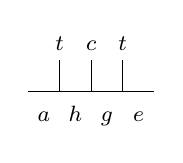
\begin{tikzpicture}[scale=0.4,font=\footnotesize,anchor=mid,baseline={([yshift=-.5ex]current bounding box.center)}]
      \draw (1, 0) to (1, -1);
      \draw (2, 0) to (2, -1);
      \draw (3, 0) to (3, -1);
      \node at (1, 0.5) {$t$};
      \node at (2, 0.5) {$c$};
      \node at (3, 0.5) {$t$};
      \draw (0, -1) to (4, -1);
      \node at (0.5, -1.75) {$a$};
      \node at (1.5, -1.75) {$h$};
      \node at (2.5, -1.75) {$g$};
      \node at (3.5, -1.75) {$e$};
    \end{tikzpicture}.
  \end{aligned}
\end{equation}
Thus, we have the following theorem.

\begin{theorem}\label{thm:general Up}
  In a given abstract anyon model, exchange of a pair of $t$-anyons around $p$ enclosed $t$-anyons is described by the exchange operator $U_p$ given by
  \begin{equation}
    U_p = \bigoplus_{c} U_{1,c}
  \end{equation}
  where $U_{1,c}$ denotes the exchange operator for two $t$ anyons around one anyon of type $c$, and $c$ ranges over all possible total charges of the $p$ enclosed anyons, that is, the possible total charges $c$ for the fusion space $V_{t^p}^c$. $U_{1,c}$ is given by
  \begin{equation}
    \begin{aligned}
      U_{1,c} \left( \fs{t,c,t}{a,b,d,e} \right) =
      \begin{tikzpicture}[scale=0.4,font=\footnotesize,anchor=mid,baseline={([yshift=-.5ex]current bounding box.center)}]
        \braid s_1^{-1} s_2^{-1} s_1^{-1};
        \node at (1, 0.5) {$t$};
        \node at (2, 0.5) {$c$};
        \node at (3, 0.5) {$t$};
        \draw (0, -3.5) to (4, -3.5);
        \node at (0.5, -4.25) {$a$};
        \node at (1.5, -4.25) {$b$};
        \node at (2.5, -4.25) {$d$};
        \node at (3.5, -4.25) {$e$};
      \end{tikzpicture} =
      \sum_{f,g,h} \left( B_{act}^d \right)_{fb} \left( B_{ftt}^e \right)_{gd} \left( B_{at c}^g \right)_{hf}
      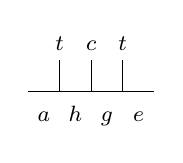
\begin{tikzpicture}[scale=0.4,font=\footnotesize,anchor=mid,baseline={([yshift=-.5ex]current bounding box.center)}]
        \draw (1, 0) to (1, -1);
        \draw (2, 0) to (2, -1);
        \draw (3, 0) to (3, -1);
        \node at (1, 0.5) {$t$};
        \node at (2, 0.5) {$c$};
        \node at (3, 0.5) {$t$};
        \draw (0, -1) to (4, -1);
        \node at (0.5, -1.75) {$a$};
        \node at (1.5, -1.75) {$h$};
        \node at (2.5, -1.75) {$g$};
        \node at (3.5, -1.75) {$e$};
      \end{tikzpicture}.
    \end{aligned}
  \end{equation}
\end{theorem}





































\section{Abelian representations: Abelian anyons}

In this section we show how abelian anyons are modeled in the framework of abstract anyon models. First, note that abelian anyons are characterized by that each fusion has a unique result, i.e.\ fusion of $a$ with $b$ results in a unique label $c$ for all $a$ and $b$,
\begin{equation}
  a \times b = c.
\end{equation}
As a consequence of this we have that any fusion space of abelian anyons is trivial and one-dimensional. All intermediate charges are uniquely determined by the simple fusion rules.

As a first example we shall see how fermionic statistics fits into the framework of abstract anyon models. In the computations, recall that $R_{ab}^c = R_{ba}^c$. In this section we deviate from our convention and denote the trivial particle by $0$ and positive integers denote non-trivial label, the reason being that fusion is defined as the sum of the labels.

\begin{example}[$\mathbb{Z}_2^{(n)}$]
  Let the set of anyonic charges be $\mathbb{Z}_2 = \{0, 1\}$, the trivial vacuum particle $0$ and one non-trivial particle $1$, with corresponding fusion corresponding to addition in $\mathbb{Z}_2$, in particular
  \begin{equation}
    1 × 1 = 0.
  \end{equation}
  Since the fusion spaces are trivial, we take $F_{abc}^{a+b+c} = 1$ for all $a, b$ and $c$. Thus, the pentagon equation \cref{eq:pentagon} is trivial and the hexagon equation \cref{eq:hexagon} reduces to
  \begin{equation}
    \begin{aligned}
      % R_{ab}^{a+b} R_{ac}^{a+c} = \sum_d R_{ad}^{b+c}.
      R_{ac}^g \left(F_{bac}^d\right)^g_e R_{ab}^e &= \sum_{f} \left(F_{bca}^d\right)^g_f R_{af}^d \left(F_{abc}^d\right)^f_e \\
      \iff
      R_{ac}^{a+c} R_{ab}^{a+b} &= \sum_{f} R_{af}^{a+b+c}.
    \end{aligned}
  \end{equation}
  We have $d = a + b + c$ from the $F$ symbol $\left(F_{bac}^d\right)$, this gives $a + f = a + b + c$, i.e.\ $f = b + c$. The hexagon equation is thus reduced to
  \begin{equation}
    R_{ac}^{a+c} R_{ab}^{a+b} = R_{a,(b+c)}^{a+b+c}.
  \end{equation}
  Since $R_{ab}^{a+b} = 1$ if $a$ or $b$ equals $0$. The only non-trivial case is
  \begin{equation}
    R_{11}^{0} R_{11}^{0} = 1 \quad \iff \quad R_{11}^{0} = ±1.
  \end{equation}
  Thus, the chosen model, i.e.\ charges and fusion modeled by $\mathbb{Z}_2$ gives two distinct abelian anyon models which we parametrize by $n = 0, 1$ so that we have
  \begin{equation}
    R_{11}^0 = e^{inπ}.
  \end{equation}
  We denote these two models by $\mathbb{Z}_2^{(n)}$ for $n = 0, 1$. In conclusion, we see that fermionic statistics are modeled by $\mathbb{Z}_2^{(1)}$. Similarly, bosonic statistics is modeled by $\mathbb{Z}_2^{(0)}$.
\end{example}

In the above example we considered fusion modeled by $\mathbb{Z}_2$ and saw that this gives rise to two distinct models. Before stating the general result, we first extend the example to see more clearly how the hexagon equation determines the $R$ matrices.

\begin{example}[$\mathbb{Z}_3^{(n)}$]
  Let fusion be modeled on $\mathbb{Z}_3$, so that the charge label set is $\mathbb{Z}_3 = \{0, 1, 2\}$ and fusion is given by addition modulo 3,
  \begin{equation}
    a \times b = [a + b]_3.
  \end{equation}
  The only non-trivial instances of the hexagon equation are
  \begin{equation}
    \begin{aligned}
      \left( R_{11}^2 \right)^2 &= R_{12}^0 \\
      \left( R_{12}^2 \right)^2 &= R_{11}^2 \\
      \left( R_{22}^1 \right)^2 &= R_{12}^2 \\
      R_{11}^2 R_{12}^0 &= 1 \\
      R_{12}^0 R_{22}^1 &= 1.
    \end{aligned}
  \end{equation}
  The first two equations combined give $\left( R_{11}^2 \right)^3 = 1 \iff R_{11}^2 = e^{i2πn/3}$. Each of the three solutions for $R_{11}^2$, corresponding to $n = 0, 1, 2$ give a solution for $R_{12}^2$ and $R_{22}^1$. This gives rise to three distinct models:
  \begin{itemize}
    \item $\mathbb{Z}_3^{(0)}$: The trivial solution $R_{ab}^{a+b} \equiv 1$ for all $a, b$.
    \item $\mathbb{Z}_3^{(1)}$: Take $R_{11}^2 = e^{i2π/3}$, the fourth equation gives $R_{12}^0 = e^{i4π/3}$ and the fifth equation gives $R_{22}^1 = e^{i2π/3}$.
    \item $\mathbb{Z}_3^{(2)}$: Take $R_{11}^2 = e^{i4π/3}$, the fourth equation gives $R_{12}^0 = e^{i2π/3}$ and the fifth equation gives $R_{22}^1 = e^{i2π/3}$.
  \end{itemize}
  The possible solutions can be compactly written as
  \begin{equation}
    R_{ab}^{a+b} = e^{i\frac{2πn}{3}ab}
  \end{equation}
\end{example}

Indeed, the more general result holds, discussed further in \cite{bonderson}, motivating the following definition.

\begin{definition}
  The abelian model $\mathbb{Z}_N^{(n)}$ is given by taking the charge label set to be $\mathbb{Z}_N$ and fusion given by addition modulo $N$,
  \begin{equation}
    a \times b = [a + b]_N.
  \end{equation}
  In this model we have
  \begin{align}
    \label{eq:abelian F}
    F_{abc}^{a+b+c} &\equiv 1 \\
    \label{eq:abelian R}
    R_{ab}^{a+b} &= e^{i\frac{2πn}{N}ab}.
  \end{align}
  By \cref{def:B} we thus have
  \begin{align}\label{eq:abelian B}
    B_{abc}^{a+b+c} = R_{bc}^{b+c},
  \end{align}
  note that the left charge $a$ does not enter the expression.
\end{definition}

Consider $\mathbb{Z}_N^{(n)}$ and the fusion space $\widetilde{V}_{1^m}$ which now is one-dimensional containing one standard fusion state
\begin{equation}
  \fswideflex{1,1}{a,a+1,a+2}{3} \ldots \fswideflex{1,1}{a+m-1,a+m,a+m+1}{5}
\end{equation}
where $a$ is any charge in $\mathbb{Z}_N$ representing the fact that the $m$ considered anyons may be part of a larger set of anyons. In \cref{res:sigma j is B} we showed
\begin{align}
  ρ(σ_j) = B_{b_{j-2} a_j a_{j+1}}^{b_j}.
\end{align}
\Cref{eq:abelian B,eq:abelian R} reduces this to
\begin{align}
  ρ(σ_j) = R_{11}^2 = e^{i\frac{2πn}{N}}
\end{align}
for all $j$. This precisely models abelian anyons with anyonic phase $α = \frac{2n}{N}$, i.e.\ any fractional phase. What we have obtained here precisely corresponds to the discussion of abelian anyons in \cref{sec:statistical repulsion abelian ayons} which was treated before we had the general framework of abstract anyon models.

Furthermore, in the fusion space $\widetilde{V}_{1^m}$ of the $\mathbb{Z}_N^{(n)}$ model, the exchange operator $U_p$ is
\begin{equation}
  \begin{aligned}
    U_p &=
    ρ(σ_1) ρ(σ_2) \cdots ρ(σ_p) ρ(σ_{p+1}) ρ(σ_p) \cdots ρ(σ_2) ρ(σ_1) \\
    &= \left( ρ(σ_1) \right)^{2p+1} = e^{i(2p+1)α}.
  \end{aligned}
\end{equation}
\Cref{thm:general Up} is clearly not needed in the abelian case, we instantly have all information of $U_p$. However, \cref{thm:general Up} still applies, first change basis to the fused basis
\begin{gather*}
  \fswideflex{1,1}{a,a+1,a+2}{3} \cdots \fswideflex{1,1}{a+p+1,a+p+2,a+p+3}{5} \\
  \xmapsto{F}
  \fswideflex{1,p,1}{a,a+1,a+p+1,a+p+2}{5}
\end{gather*}
and \cref{thm:general Up} gives
\begin{align}
  U_p \left( \fs{1,c,1}{a,b,d,e} \right) =
  \sum_{f} \left( B_{act}^d \right)_{fb}
  \sum_{g} \left( B_{ftt}^e \right)_{gd}
  \sum_{h} \left( B_{at c}^g \right)_{hf}
  \fs{1,c,1}{a,h,g,e}.
\end{align}
As we've seen, the intermediate charges play no role, indeed the fusion space is one-dimensional. In the $\mathbb{Z}_N^{(n)}$model this expression for $U_p$ immediately reduces to
\begin{align}
  U_p =
  R_{c1} R_{11} R_{1c} =
  e^{ipαπ} e^{iαπ} e^{ipαπ} =
  e^{i(2p+1)απ}
\end{align}
as expected.
